% =====================================================================
%  Schéma du bus CAN du cobot : deux moteurs RMD (MyActuator) aux extrémités,
%  une Nucleo-L476RG avec transceiver en dérivation. Sans PC ni CANable.
%  Même charte de couleurs que le dossier du banc de test.
%  Compilation : pdflatex schema_bus_cobot.tex
% =====================================================================
\documentclass[border=8pt]{standalone}
\usepackage[utf8]{inputenc}
\usepackage[T1]{fontenc}
\usepackage{xcolor}
\usepackage{siunitx}
\usepackage{tikz}
\usetikzlibrary{positioning,arrows.meta,calc}
\sisetup{locale=FR}

\definecolor{canh}{RGB}{200,30,30}
\definecolor{canl}{RGB}{30,60,200}
\definecolor{nodefill}{RGB}{240,244,250}
\definecolor{mcufill}{RGB}{220,235,255}
\definecolor{trxfill}{RGB}{255,240,215}
\definecolor{termfill}{RGB}{245,225,225}
\definecolor{grey}{RGB}{105,105,105}

\tikzset{
  motor/.style={draw, rounded corners=3pt, fill=nodefill, line width=1pt},
  block/.style={draw, line width=0.6pt, align=center, font=\small, minimum height=1.25cm, inner sep=3pt},
  mcu/.style={block, fill=mcufill},
  trx/.style={block, fill=trxfill},
  term/.style={draw, line width=0.8pt, fill=termfill, minimum width=0.42cm, minimum height=0.5cm},
  lbl/.style={font=\small, text=grey, align=center},
  busH/.style={canh, line width=2.2pt},
  busL/.style={canl, line width=2.2pt},
  thin/.style={line width=0.6pt},
}

% Un moteur : boîte, contrôleur, transceiver.
% #1 abscisse du centre, #2 sens (+1 : bus à droite, -1 : bus à gauche), #3 nom, #4 référence
\newcommand{\motor}[4]{%
  \node[motor, minimum width=8.4cm, minimum height=3.5cm] (#3) at (#1,0) {};
  \node[font=\large\bfseries, anchor=south] at ($(#3.north)+(0,-0.66)$) {#4};
  \node[mcu, text width=1.5cm] (#3m) at ({#1-#2*3.15},0) {Contrôleur moteur};
  \node[trx, text width=1.5cm] (#3t) at ({#1-#2*0.95},0) {Transceiver CAN};
}

\begin{document}
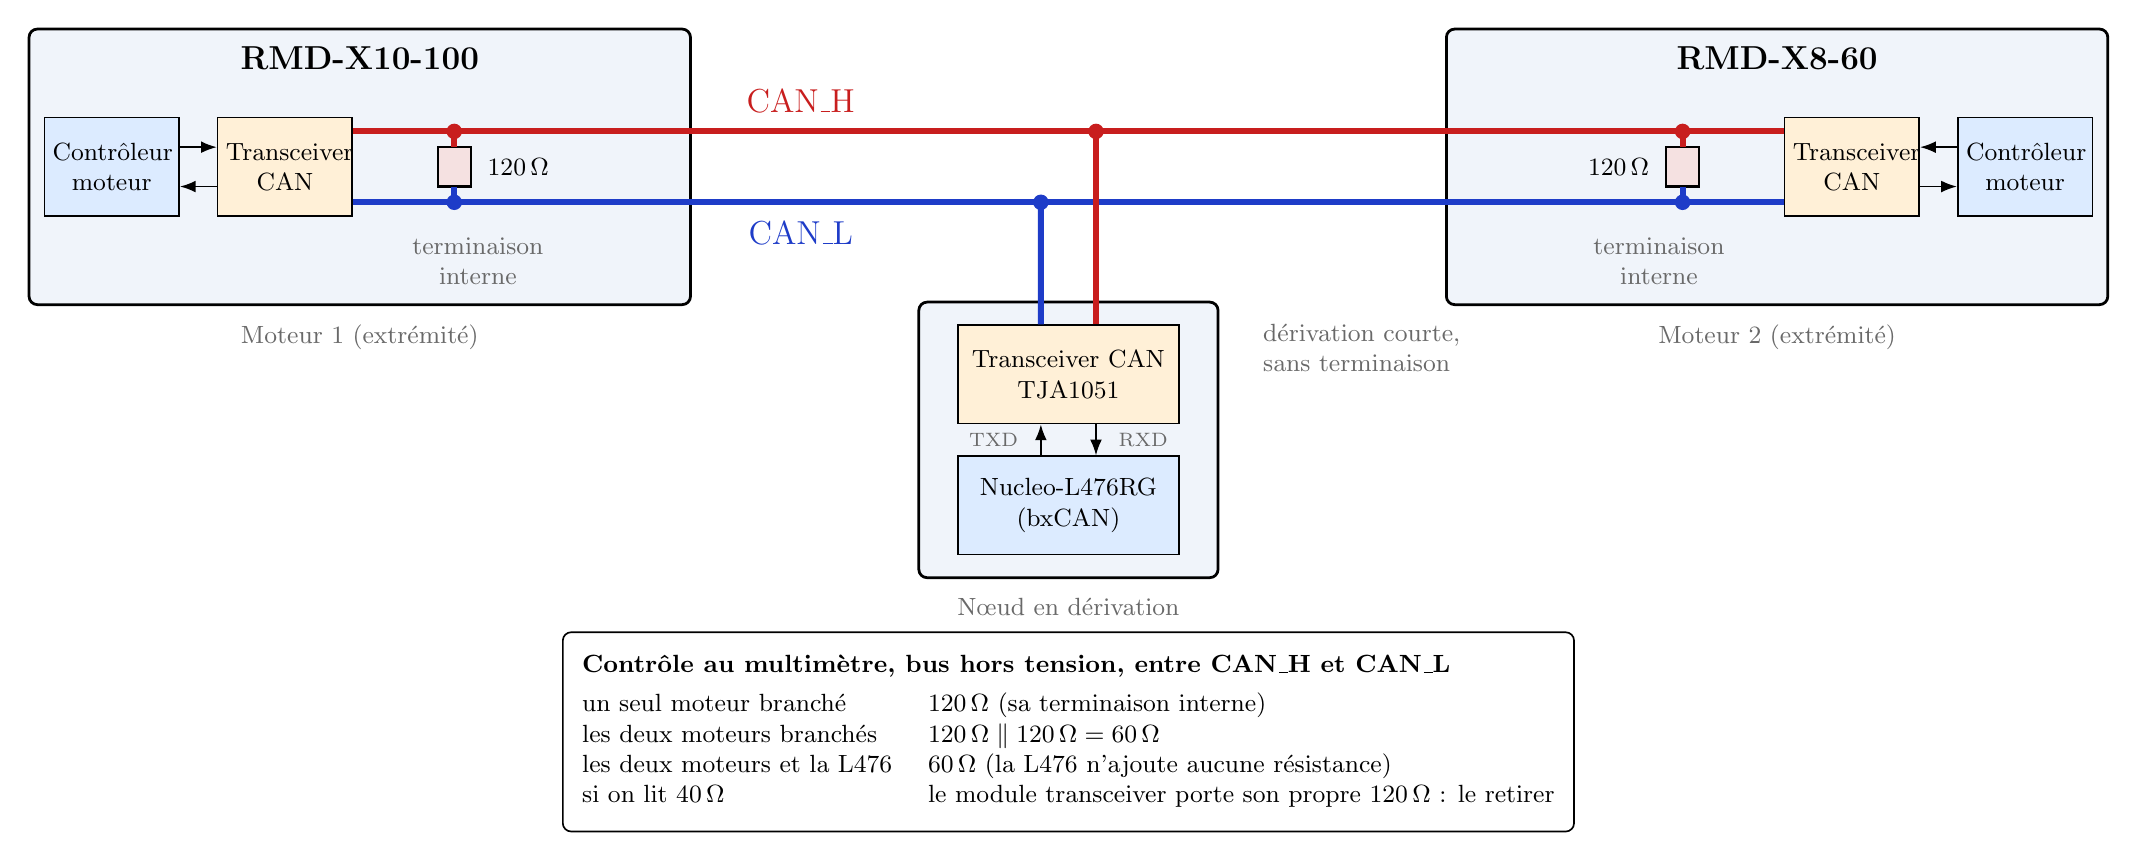
\begin{tikzpicture}[x=1cm,y=1cm]

% --- Géométrie : les deux moteurs sont les deux extrémités du bus ------------------
\def\yH{0.45}    % CAN_H
\def\yL{-0.45}   % CAN_L
\def\xB{18}      % centre du moteur 2
\def\xC{9}       % centre de la L476

\motor{0}{1}{A}{RMD-X10-100}
\motor{\xB}{-1}{B}{RMD-X8-60}
\node[lbl, anchor=north] at ($(A.south)+(0,-0.12)$) {Moteur 1 (extrémité)};
\node[lbl, anchor=north] at ($(B.south)+(0,-0.12)$) {Moteur 2 (extrémité)};

% liaisons contrôleur - transceiver des moteurs
\draw[thin, -{Latex[length=2mm]}] ($(Am.east)+(0,0.25)$) -- ($(At.west)+(0,0.25)$);
\draw[thin, {Latex[length=2mm]}-] ($(Am.east)+(0,-0.25)$) -- ($(At.west)+(0,-0.25)$);
\draw[thin, -{Latex[length=2mm]}] ($(Bm.west)+(0,0.25)$) -- ($(Bt.east)+(0,0.25)$);
\draw[thin, {Latex[length=2mm]}-] ($(Bm.west)+(0,-0.25)$) -- ($(Bt.east)+(0,-0.25)$);

% --- Le bus : deux fils d'un moteur à l'autre ------------------------------------
\draw[busH] (At.east |- 0,\yH) -- (Bt.west |- 0,\yH);
\draw[busL] (At.east |- 0,\yL) -- (Bt.west |- 0,\yL);

% --- Terminaisons internes des moteurs : une résistance entre CAN_H et CAN_L -------
\foreach \x in {1.2, 16.8} {
  \node[term] at (\x,0) {};
  \draw[busH] (\x,0.25) -- (\x,\yH);
  \draw[busL] (\x,-0.25) -- (\x,\yL);
  \fill[canh] (\x,\yH) circle (2.8pt);
  \fill[canl] (\x,\yL) circle (2.8pt);
}
\node[font=\small, anchor=west] at (1.5,0) {\SI{120}{\ohm}};
\node[font=\small, anchor=east] at (16.5,0) {\SI{120}{\ohm}};
\node[lbl, text width=2.4cm] at (1.5,-1.2) {terminaison interne};
\node[lbl, text width=2.4cm] at (16.5,-1.2) {terminaison interne};

% --- Nucleo-L476RG : nœud en dérivation, sans terminaison -------------------------
\node[motor, minimum width=3.8cm, minimum height=3.5cm, anchor=north] (C) at (\xC,-1.7) {};
\node[trx, text width=2.6cm, anchor=north] (Ct) at ($(C.north)+(0,-0.3)$) {Transceiver CAN\\ TJA1051};
\node[mcu, text width=2.6cm, anchor=south] (Cm) at ($(C.south)+(0,0.3)$) {Nucleo-L476RG\\ (bxCAN)};
\draw[thin, -{Latex[length=2mm]}] ($(Cm.north)+(-0.35,0)$) -- ($(Ct.south)+(-0.35,0)$);
\draw[thin, {Latex[length=2mm]}-] ($(Cm.north)+(0.35,0)$) -- ($(Ct.south)+(0.35,0)$);
\node[font=\scriptsize, text=grey] at ($(Ct.south)!0.5!(Cm.north)+(-0.95,0)$) {TXD};
\node[font=\scriptsize, text=grey] at ($(Ct.south)!0.5!(Cm.north)+(0.95,0)$) {RXD};
\node[lbl, anchor=north] at ($(C.south)+(0,-0.12)$) {Nœud en dérivation};

% dérivation courte : un fil vers CAN_H, un fil vers CAN_L
\draw[busH] ($(Ct.north)+(0.35,0)$) -- (\xC+0.35,\yH);
\draw[busL] ($(Ct.north)+(-0.35,0)$) -- (\xC-0.35,\yL);
\fill[canh] (\xC+0.35,\yH) circle (2.8pt);
\fill[canl] (\xC-0.35,\yL) circle (2.8pt);

% --- Étiquettes du bus ---------------------------------------------------------------
\node[font=\large, text=canh, anchor=south] at (5.6,0.57) {CAN\_H};
\node[font=\large, text=canl, anchor=north] at (5.6,-0.57) {CAN\_L};
\node[lbl, anchor=west, text width=3.4cm, align=left] at (\xC+2.35,-2.3) {dérivation courte,\\ sans terminaison};

% --- Contrôle attendu ----------------------------------------------------------------
\node[draw, rounded corners=3pt, line width=0.6pt, font=\small, anchor=north, inner sep=7pt] at (9,-5.9) {%
  \begin{tabular}{@{}l@{\hspace{1.4em}}l@{}}
    \multicolumn{2}{@{}l@{}}{\textbf{Contrôle au multimètre, bus hors tension, entre CAN\_H et CAN\_L}}\tabularnewline[3pt]
    un seul moteur branché & \SI{120}{\ohm} (sa terminaison interne)\tabularnewline
    les deux moteurs branchés & $\SI{120}{\ohm}\parallel\SI{120}{\ohm} = \SI{60}{\ohm}$\tabularnewline
    les deux moteurs et la L476 & \SI{60}{\ohm} (la L476 n'ajoute aucune résistance)\tabularnewline
    si on lit \SI{40}{\ohm} & le module transceiver porte son propre \SI{120}{\ohm} : le retirer
  \end{tabular}};

\end{tikzpicture}
\end{document}
